\hypertarget{index_Introduction}{}\section{Introduction}\label{index_Introduction}
Determining dead and noisy channels is based on the analysis of the channel ADC spectra recorded during a PMNoiseRun. These spectra are provided by {\ttfamily ahcBinHst} from the {\ttfamily calice\_\-daq} package.

 
\begin{DoxyImage}
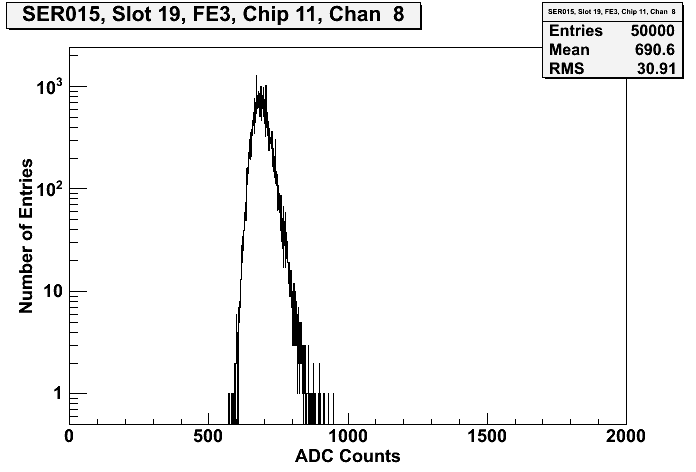
\includegraphics[width=0.7\textwidth]{normal_channel_spectrum.png}
\caption{Typical ADC spectrum of a channel in a noise run.}
\end{DoxyImage}


Only the mean of the distribution (the pedestal in case of a noise run) and the width (RMS) are used.\hypertarget{index_Definition}{}\section{Definition of dead and noisy}\label{index_Definition}
Currently dead and noisy are only defined from the RMS. \hypertarget{index_Noisy}{}\subsection{Noisy}\label{index_Noisy}
Looking at RMS sectrum of all channels one sees that most channels have an RMS around 40, but some channels (the noisy ones) have much larger RMS, causing a tail in the distribution.

 
\begin{DoxyImage}
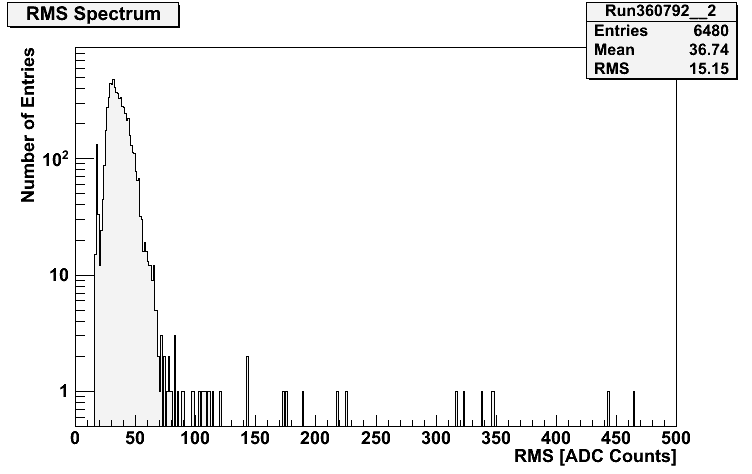
\includegraphics[width=0.7\textwidth]{rms_spectrum.png}
\caption{The RMS spectrum of all channels.}
\end{DoxyImage}


{\bfseries Definiton of noisy: RMS $>$ 140 }\hypertarget{index_Dead}{}\subsection{Dead}\label{index_Dead}
A comparisan with data and LEDVCalib runs has shown that the peak at the lover end of the distribution contains basically only dead channels (see section \char`\"{}Comparing two runs\char`\"{}).

 
\begin{DoxyImage}
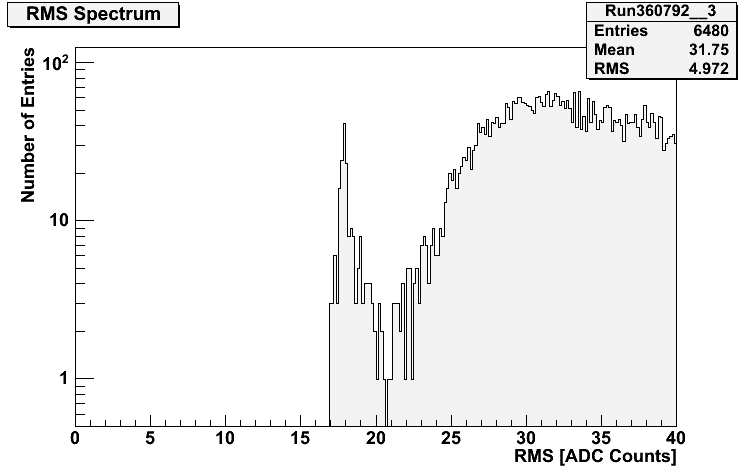
\includegraphics[width=0.7\textwidth]{rms_spectrum_zoom.png}
\caption{The RMS spectrum of all channels.}
\end{DoxyImage}


{\bfseries Definiton of dead: RMS $<$ 20.5 }\hypertarget{index_SWOverview}{}\section{Software overview}\label{index_SWOverview}
The software basically consists of two parts \begin{DoxyItemize}
\item The root library {\ttfamily libDeadAndNoisyTools} which conveniently allows to access the RMS and pedestal values of one or several runs \item The {\ttfamily createBadChannelsList} executable which creates the list of bad channels to be written to the database.\end{DoxyItemize}
\hypertarget{index_pages}{}\subsection{Detailed descritons}\label{index_pages}
\begin{DoxyItemize}
\item \hyperlink{downloadinstall}{Download and Installation} \item The \hyperlink{createbadchannelslist_exe}{createBadChannelsList} executable \item The \hyperlink{rootlib}{libDeadAndNoisyTools} root library \item \hyperlink{examples}{Examples}\end{DoxyItemize}
\hypertarget{index_Outlook}{}\section{Outlook}\label{index_Outlook}
\begin{Desc}
\item[\hyperlink{todo__todo000007}{Todo}]Implement convenience draw functions which create the default plots with well formated axis labels etc. 

Transfer missing functionality from C scripts. 

Maybe implement GUI?\end{Desc}
